\section{Cast your soul to the sea}


\begin{wrapfigure}{rt}{.3\textwidth}
 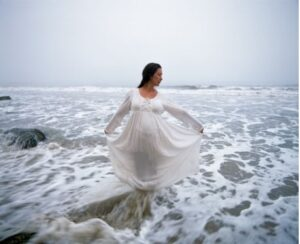
\includegraphics[scale=.5]{a20220517Castyoursoultothesea-img001.jpg}
\end{wrapfigure}

\textbf{Loreena McKennitt} composed the song Dante's Prayer while riding the Trans-Siberian Railway after the fall of the Soviet Union. The barren landscape inspired the poem. The \textbf{St. Petersburg Chamber Choir} performed a piece entitled \textit{Alleluia, Behold the Bridegroom} in the first recording of the song.

The poem begins in the woods, rises through the mountains, and flies to touch the face of the stars.

\begin{verse}
\textit{Dante's Prayer} by \textbf{Loreena McKennitt}\\
When the dark wood fell before me\\
And all the paths were overgrown\\
When the priests of pride say there is no other way\\
tilled the sorrows of stone.

I did not believe because I could not see\\
Though you came to me in the night\\
When the dawn seemed forever lost\\
You showed me your love in the light of the stars.

Cast your eyes on the ocean\\
Cast your soul to the sea\\
When the dark night seems endless\\
Please remember me.

Then the mountain rose before me\\
By the deep well of desire\\
From the fountain of forgiveness\\
Beyond the ice and the fire.

Cast your eyes on the ocean\\
Cast your soul to the sea\\
When the dark night seems endless\\
Please remember me.

Though we share this humble path, alone\\
How fragile is the heart\\
Oh give these clay feet wings to fly\\
To touch the face of the stars.

Breathe life into this feeble heart\\
Lift this mortal veil of fear\\
Take these crumbled hopes, etched with tears.\\
We'll rise above these earthly cares.

Cast your eyes on the ocean\\
Cast your soul to the sea\\
When the dark night seems endless\\
Please remember me,\\
Please remember me.
\end{verse}

\url{https://www.youtube.com/watch?v=KC2cCNspS1M}
\flrightit{Posted on 2022-05-17 by Cologero }
